\documentclass{mcmthesis}
\mcmsetup{CTeX = false,   % 使用 CTeX 套装时,设置为 true
        tcn = 55869, problem = E,
        sheet = true, titleinsheet = true, keywordsinsheet = true,
        titlepage = false, abstract = true}
\problem{E}

\makeatletter % `@' now normal "letter"   %follpw as section test
\@addtoreset{equation}{section}
\makeatother  % `@' is restored as "non-letter"
\renewcommand\theequation{\oldstylenums{\thesection}%
                   .\oldstylenums{\arabic{equation}}}

\usepackage{palatino}
\usepackage{mwe}
\usepackage{graphicx}
\usepackage{tabularx}
\usepackage{float}
\usepackage{indentfirst}
\usepackage{amsmath}
\usepackage{caption}
\usepackage{subfigure}
\title{}
\date{}

\begin{document}

\begin{abstract}%摘要


\title{Keep the Bathtub Warm}
\indent In this paper, we focus on the need for keeping the initial temperature of the water in the bathtub without a secondary heating system and circulating jets as much as possible. We build a model of the temperature of the bathtub water in space and time , analysis the impact of the bathtub's volume, shape and factors of people, then make a non-technical statement.\\
\indent
Our model is mainly based on the loss and inflow of heat and variety of the amount of water.\\
\indent
First, using the heat conduction formula, the heat convection formula and the formula of water surface evaporation, we build a basic heat dissipation model, including the dissipation of the surface of water and interface between water and bathtub. Due to the input of heat depends on the input of water, we build two models based on different ways of water adding. The first type is to add water by manual adjustment, while the second type is to adjust the water automatically by PID. For the variety of the amount of water, we limit the ceiling of water and build a basic drainage model.\\
\indent
The model is simulated and verified by the statistics and results. As for the first type-add hot water, we determine an appropriate water flow rate per unit time, to make temperature fluctuations remain within the range ($0.1^{\circ}C$ ). We simulate the degradation to figure out the approximate optimal solution, which results in a more stable temperature and less waste. As for the second type, we adjust the PID index and build a more stable model, in which the temperature remains unchanged almost, the amount of water reduce by 8-13\% compared with manual adjustment. Considering the random water flow spillover, we simulate two models and validate the stability.\\
\indent
The model is improved in consideration of the size of human body, movement and body temperature. The relation between body size and surface area and height and weight was obtained by using data and empirical formula. Because the internal temperature of human is kept constant, we add the heat absorption model to the heat dissipation model using Newton's law of cooling. In the model of the water change, we add the impact of body volume on the level of the water, and the amount of water overflow that may occur due to the movement of people.\\
\indent
Bubble is considered to influence mainly heat loss model. We calculate the reflection coefficient to modify the value of radiation in heat loss model. Because the air in the bubble will be saturated in a short time, we ignore the evaporation in the heat loss model.\\
\indent
We simulate under different conditions, give the results. And the effects of different factors are compared and analyzed. Finally, we give the strengths and weaknesses of our models. \\


\begin{keywords}
 \textbf{Heat dissipation model,\indent Continuous water addition model, Continues system simulation,\indent Simulate Anneal Arithmetic(SAA),\indent PID}
\end{keywords}
\end{abstract}

\maketitle
\tableofcontents\thispagestyle{empty}
%设置页眉


\setcounter{page}{1}
%Section 1
\section{Introduction}
\subsection{Background}%subsection 1.1
\indent the traditional bathtub is a simple waterproof container.
the bathtub temperature is decreasing and people need to constantly add hot water to maintain the temperature.\\
\indent We want to establish such a viable model which can automatically add hot water to keep the temperature of the bathtub at the comfort temperature. At the same time saving water resources needs to be considered.
\subsection{Our work}

\indent We want to establish such a viable model which can automatically add hot water to keep the temperature of the bathtub at the comfort temperature. At the same time saving water resources needs to be considered.\\
\indent To solve this problem, we need to consider the impact of the bathtub shape and size on this model. Person's shape,size and temperature are also under consideration.

%Section 2
\section{Assumptions}
\noindent
{\bf (1) } \textbf{Evaporation will result in no loss of water.} The loss of water from evaporation is too little to consider, so we ignore the change of quantity of water.\\
{\bf (2) } \textbf{Consider the energy of water in 36 ${^\circ}C$ as the energy reference.} For we can arbitrarily set our energy reference to be zero.\\
{\bf (3) } \textbf{加入水的温度是固定的} \\
{\bf (4) } \textbf{流出的水的温度就是浴缸的初始温度} \\
{\bf (5) } \textbf{沐浴过程中室温不变} \\


\section{Symbol Description}
\begin{table}[H]
        \setlength{\abovecaptionskip}{0pt}
        \setlength{\belowcaptionskip}{0pt}
				\centering{Table 1:Constants}\\
        \begin{tabular}{p{2cm}|p{2cm}|p{7.5cm}|p{1.7cm}}
		\hline
		\rowcolor[gray]{0.9}\bf{Symbol}	&\bf{uint}      &\bf{Meaning}&\bf{value}	\\
		\hline
		${P}''_{v}$		& $hP_{a}$		 & vapor pressure of thin saturated layer on water surface  &test\\
		$P_{v}$		& $hP_{a}$		 & water vapor partial pressure in wet air\\
		$P_{a}$		& $hP_{a}$		 & atmospheric pressure  &test\\
		$L$		& $kj/kg$		 & heat of water vaporization&2500\\
		$\varepsilon$		& 		 & emissivity&0.97\\
		$C_{p}$		& $KJ/(kg\cdot K)$		 & specific heat capacity of dry air at 300k &1.005\\
		$C_{water}$		& $KJ/(kg\cdot K)$		 & specific heat capacity of water at 300k &4.196\\

		\hline
		\end{tabular}
	\end{table}

\begin{table}[H]
        \setlength{\abovecaptionskip}{0pt}
        \setlength{\belowcaptionskip}{0pt}
        \centering{Table 2:Notation} \\
        \begin{tabular}{p{1.8cm}|p{2.2cm}|p{9cm}}
        \hline
        \rowcolor[gray]{0.9}\bf{Symbol}	&\bf{uint}      &\bf{Meaning}\\
        \hline
        $V(h)$			& $m^3  $		 & the relationship between volume of water and liquid height \\
        $S_{1}(h)$		& $m^2  $		 & the top surface area of the liquid 	\\
        $S_{2}(h)$		& $m^2  $		 & the lower surface area of the bathtub 	\\
        $S_{3}(h)$		& $m^2  $		 & the side contact area of the bathtub and liquid 	\\
        \emph{S}	& $m^2  $		 & the surface area of the body\\
        ${h_{p}}$	& $cm	$        & height of a person \\
        \emph{w}	& $kg	$        & weight of a person \\
        $\alpha$		& $ W/(m^{2}\cdot^{\circ}C)  $		 & heat dissipation coefficient\\
        $t$		& $ ^{\circ}C  $		 & surface temperature of water \\
        $\theta$		& $^{\circ}C$		 & dry bulb temperature of air\\
        $\beta$		& $W/(m^{2}\cdot hP_{a})$		 & evaporation coefficient\\
        $Q_{upper}$		& $J$		 & bathtub top surface unit time heat dissipation\\
		$Q_{side}$		& $J$		 & bathtub side surface unit time heat dissipation\\
		$t_{in}$		& ${^\circ}C$		 & the temperature of the water poured in\\
		$Q_{in}$		& $J$		 & the energy brought into the bathtub in period of time \\
		        \hline
        \end{tabular}
        \end{table}

%Section 3
\section{Heat Dissipation Model}
In order to analyze the situation of heat dissipation. 
We need to start from the bathtub.
The effect of a bathtub on heat loss is mainly in material and shape.\\
\indent The surface area of the liquid is variable because of the different shapes and attributes about bathtubs. Likewise the contact area of liquid and bathtub. Therefore We use functions to describe the relationship between the surface area of liquid, the liquid surface height and the contact area of liquid and bathtub. \\
\indent We use these abstract expression to avoid the effect of exact shapes and attributes on the model.
\begin{equation}
\begin{split}
h=H(v)  \\
S_{1}=S_{1}(h) \\
S_{2}=S_{2}(h)  \\
\end{split}
\end{equation}
\indent The water in the bathtub dissipates heat by contacting the air on the upper surface and the bathtub wall on the side surface. So we So we decompose the model into two parts:\\
\indent \indent1) Liquid surface heat loss model\\
\indent \indent2) contact area of liquid and bathtub heat loss model
\subsection{Liquid surface heat loss model}
\indent The water dissipation mode including three parts: evaporation heat, convection heat and radiative heat dissipation.We use the coefficient of heat dissipation and dissipation general formula to get results.
\\
\indent The evaporation heat is the amount of heat transmitted to the air by the water at unit time $Q_{a}$. It can be represented by following formula:
\begin{equation}
	dQ_{a}=\alpha (t-\theta)dS
\end{equation}
\indent The convection heat is the amount of heat that evaporates through the water at unit time $Q_{b}$. It can be represented by following formula:
\begin{equation}
	Q_{b}=\beta ({p}''_{v}-p_{v})dS
\end{equation}
\indent Radiative heat dissipation is a heat transfer method that emits light in a straight line in all directions centered on a heat source $Q_{c}$.  It can be represented by following formula:
\begin{equation}
	dQ_{c}=\varepsilon \sigma (t+273)^{4}dS
\end{equation}
\indent In unit time, the heat dissipation of the water surface is \cite{1}
\begin{equation}
 dQ=dQ_{a}+dQ_{b}+dQ_{c}=[\alpha (t-\theta)+\beta ({p}''_{v}-p_{v})+\varepsilon \sigma (t+273)^{4}]dS 
\end{equation}
\indent \indent \indent $\varepsilon$ is the emissivity. The value is 0.97\\
\indent \indent \indent $\sigma$ is a constant. The value is $5.6\times 10^{-8}$\\
\indent \indent \indent In the actual process, $\beta$ and $\alpha$ can be obtained by General formula \cite{2}:\\
\begin{equation}
 \beta=\sqrt{[22.0+12.5W^{2}+2.0(t-\theta)}
\end{equation}
\begin{equation}
 \frac{\alpha}{\beta}=b=\frac{P_{a}C_{p}}{0.623L}
\end{equation}
\indent $C_{p}$ is the specific heat capacity of dry air. As the temperature changes, there is little change in the value. So we take the value as the temperature equals to 300k.\\
\begin{equation}
C_{p}=1.005KJ/(kg\cdot K)
\end{equation}
\indent According to assumption (3), the temperature of the water has the same value. So during unit time, the total heat dissipating capacity in the upper surface is:\\
\begin{equation}
\begin{split}
Q_{upper}&=\int_{upper} dQ\\
&= \int_{upper}\alpha (t-\theta)+\beta ({p}''_{v}-p_{v})+\varepsilon \sigma (t+273)^{4}dS	\\
&=[\alpha (t-\theta)+\beta ({p}''_{v}-p_{v})+\varepsilon \sigma (t+273)^{4}]\cdot S_{1}\
\end{split}
\end{equation}

\subsection{Side area of bathtub heat loss model} 	%4.2
\indent The heat dissipated area is the contact part between bathtub and liquid.So we just need to think about the effect of contact area. \\ \indent For the water in the side surface of the bathtub is not in direct contact with the air, there will be no evaporation. Therefore there will not be $ dQ_{b} $ in the equation (4.2). Considering of the reflex of thermal radiation between water and the side surface, $dQ_{c}$ will change.\\ \indent The material of the side surface of the bathtub is acrylic. The index of refraction of acrylic is $n_{1}\approx 1.4$, the index of refraction of water is $ n_{0}\approx 1.33 $.\\ \indent So the reflection coefficient is 
\begin{equation}
	 R=\frac{(n_{0}-n_{1})^{2}}{(n_{0}+n_{1})^{2}}=\frac{(1.4-1.33)^{2}}{(1.4+1.33)^2}=0.06 
\end{equation}
\indent Then in the equation(4.2),  the $dQ_{c}$ will be multiplied by ($1-R=0.94$).  Therefore, the heat dissipating capacity during unit time in the side surface is :
\begin{equation}
	dQ=dQ_{a}+0.94dQ_{c}=[\alpha (t-\theta)+0.94\varepsilon \sigma (t+273)^{4}]dS
\end{equation}
\indent According to assumption (3), the temperature of the water has the same value. So during unit time, the total heat dissipating capacity in the side surface is :				%4.9
\begin{equation}
\begin{split}
Q_{side}&=\int_{side}dQ\\
&= \int_{side} [\alpha (t-\theta)+0.94\varepsilon \sigma (t+273)^{4}]dS	\\
&=[\alpha (t-\theta)+0.94\varepsilon \sigma (t+273)^{4}]S_{3}\\
\end{split}
\end{equation}
\subsection{The bathtub heat loss model} 	%4.2

\indent Just as we mentioned above, the water in the bathtub dissipates heat by contacting the air on the upper surface and the bathtub wall on the side surface. \\

\indent So the total heat dissipating capacity during unit time is:
\begin{equation}
	Q_{0}=Q_{upper}+Q_{side}
\end{equation}


\indent The specific forms of $Q_{upper}$ and $Q_{side}$ can be obtained from the above. 

\section{Model of hot water addition}
\subsection{Influence of inflowing water on quantity of heat and volume}
\indent First, we should establish an abstract model to describe the heating process.\\
\indent The water in the bathtub is heated by the hot water flowing into it. So we should consider the energy and the volume of water in unit time. \\
\indent Set the unit time flow of the faucet as $ V $, and the temperature of the inflow water is $ t_{in}$. Because the  heat capacity of water changes in a very small degree, we can use $0^{\circ}$ as the reference point which means the relative quantity of heat is 0.\\
\indent Compared to the energy reference, during unit time the energy of water poured in is:
\begin{equation}
	q_{in}=C\rho Vt_{in} 
\end{equation}
\indent Adding hot water is a continuous process. Then in the constant $ T_{1} $ seconds of adding hot water, the total energy brought into the bathtub is:
\begin{equation}
	Q_{in}=q_{in}T_{1}=C\rho Vt_{in}T_{1}
\end{equation}
\indent Meanwhile, the volume of water brought into the bathtub is:
\begin{equation}
	\bigtriangleup V=VT_{1} 
\end{equation}

\subsection{Add a constant flow of hot water}
In order to facilitate user operation, we give up the discrete model using complicated intermittent inflow water.
\subsection{Use automatic control algorithm to control flow velocity}
The PID algorithm is a classic automatic control algorithm. Suppose we can get relatively accurate temperatures, accurately to 0.01$^{\circ}C$. And suppose the maximum flow rate of hot water is 100ml/s.\\
\indent We can establish an automatic control equation, which includes three items of P, I and D.\\
\begin{equation}
T_{error}=T_{target}-T_{real}
\end{equation}
\indent But considering the accuracy of temperature measurement\\
\begin{equation}
	T_{error}=\begin{cases}
	&T_{target}-T_{real} \quad\text{ if }\left | T_{target}-T_{real} \right |\geq 0.01 \\ 
	&0\indent\indent\indent\indent \text{ if } \left | T_{target}-T_{real} \right |<0.01 
	\end{cases}
\end{equation}
\indent P is a proportion term
\begin{equation}
	P=Kp\times T_{error}
\end{equation}
\indent I is an integral term
\begin{equation}
	I=Ki\times \sum T_{error}
\end{equation}
and the function of I is to Eliminate static error.\\
\indent D is a differential term.
\begin{equation}
D=Kd\times (T_{error}-T_{last_error})
\end{equation}
The function of D is to Forecast the change trend.\\
\begin{figure}[H]
\centering
\subfigure[When Kp is too small]{
\begin{minipage}{7cm}
\centering 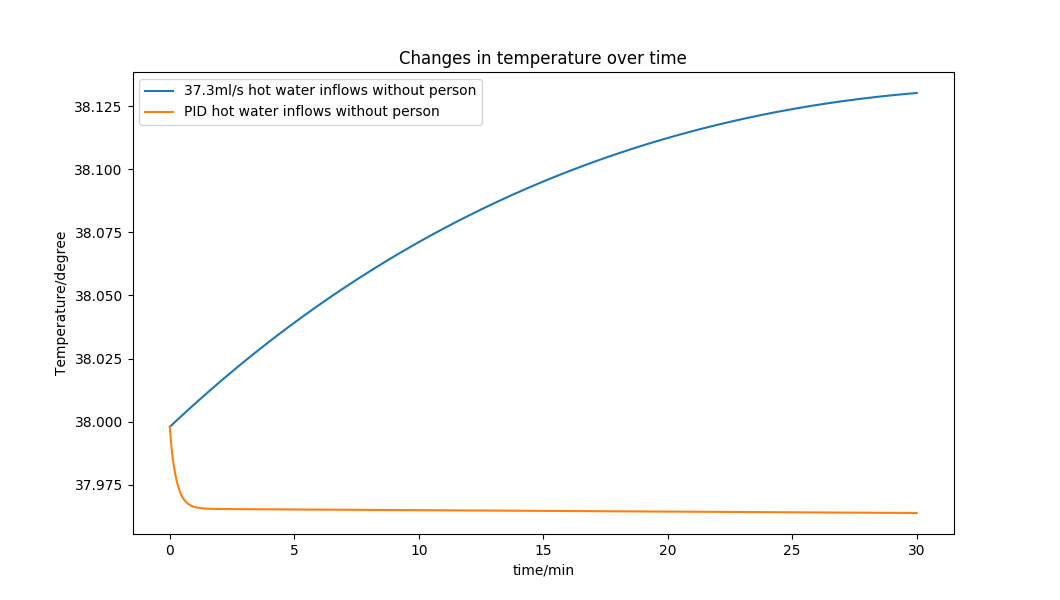
\includegraphics[scale=0.26]{PID_1.png}       
\end{minipage}
}
\subfigure[When Kp is too large]{
\begin{minipage}{7cm}
\centering                                    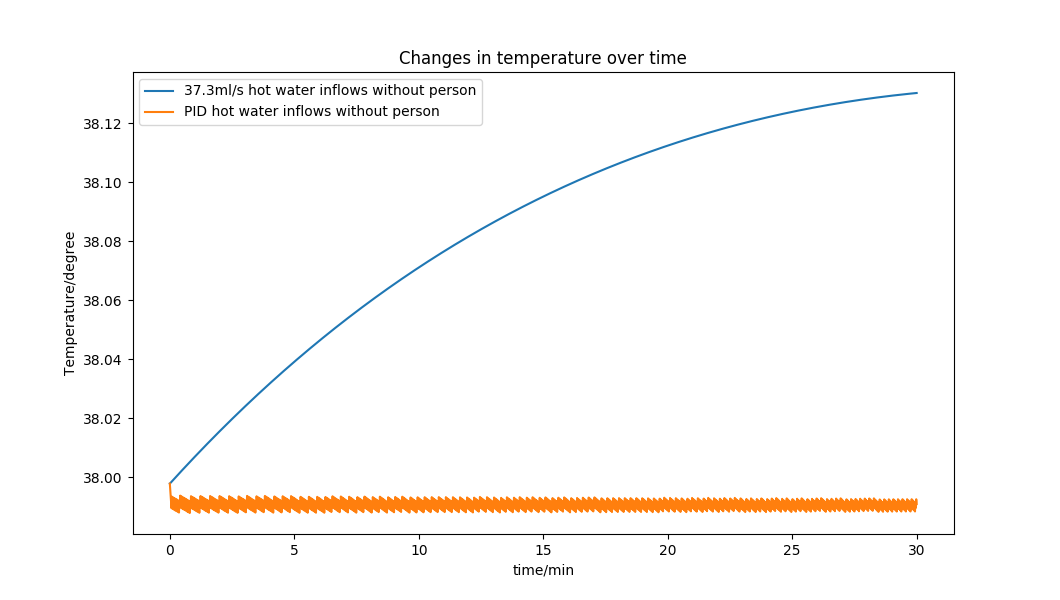
\includegraphics[scale=0.26]{PID_4.png}        
\end{minipage}
}
\caption{Only use Kp}
\label{PID1}
\end{figure}


\indent We found that only the use of P is not a good way to adjust the temperature of the water. For example, the subgraph (a) in figure \ref{PID1} shows the situation when Kp is small. There is a static difference between the expected temperature and the actual temperature. So we need to increase the value of Kp.\\
\indent The subgraph (b) in figure \ref{PID1} shows when the Kp is increased, the temperature produces a high frequency shock\\

\begin{figure}[H]
\centering
\subfigure[When Kp is too small]{
\begin{minipage}{7cm}
\centering 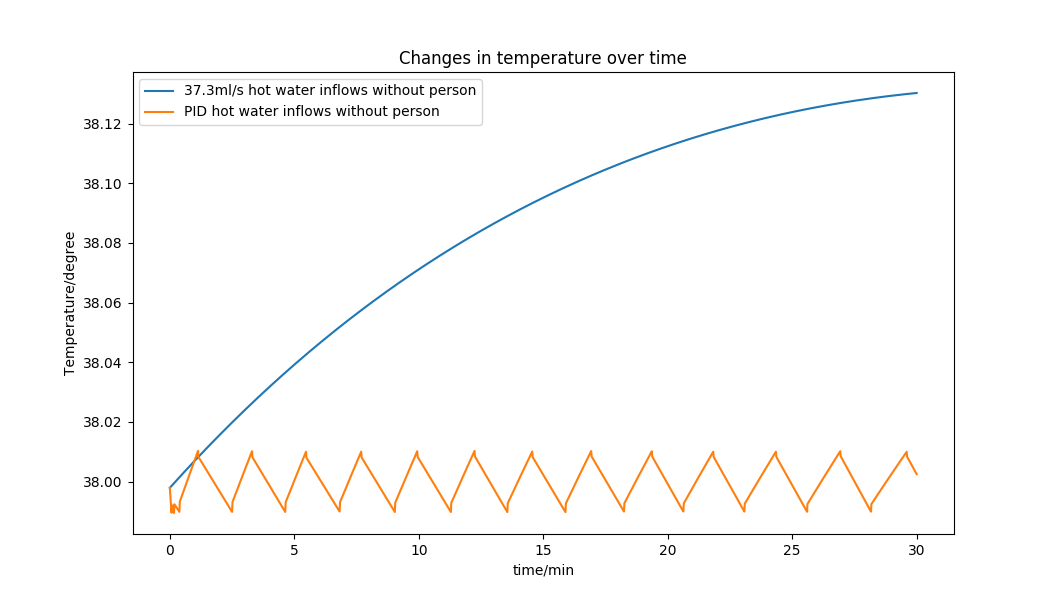
\includegraphics[scale=0.26]{PID_2.png}       
\end{minipage}
}
\subfigure[When Kp is too large]{
\begin{minipage}{7cm}
\centering                                    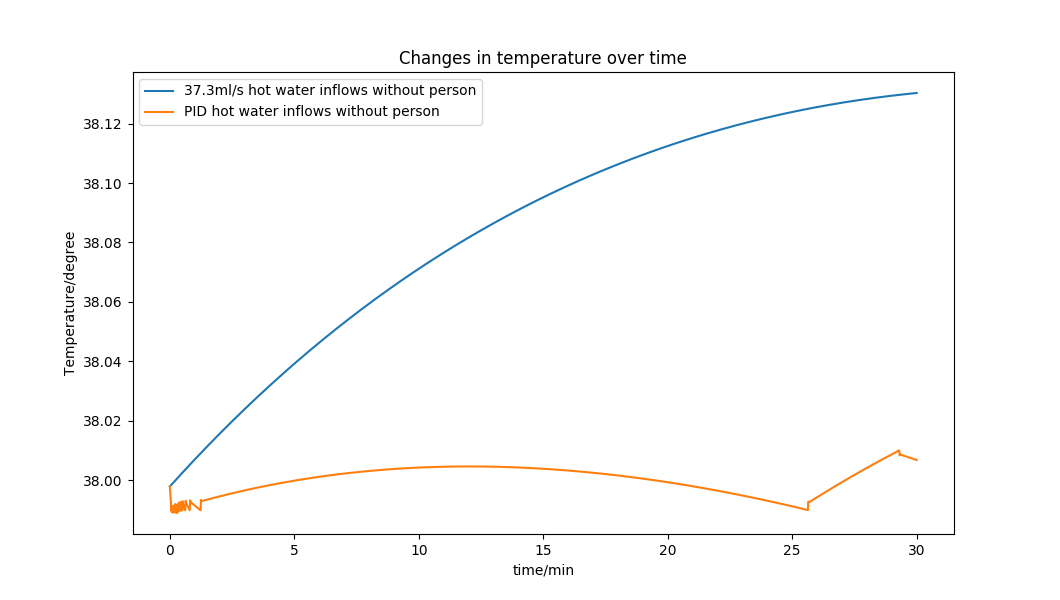
\includegraphics[scale=0.26]{PID_3.png}        
\end{minipage}
}
\caption{Use Kp, Ki, Kd}
\label{PID2}
\end{figure}
\indent We introduce the I and D items to reduce the frequency of the shock and make the water temperature as stable as possible. The subgraph (a) in figure \ref{PID2} shows when we introduce I, the static difference can be eliminated. \\
\indent The subgraph (b) in figure \ref{PID2} shows when we also introduce the D item at the same time. The temperature trend becomes more stable.\\
\section{Solutions for tasks}
\subsection{Model Implementation with Computer}
\indent In the above, We've got a general model of heating and heat loss. Take advantage of the two general models we have already obtained, we established a simulation program built with python. It can simulate the process of heating and heat loss. We can use the simulation program to solve the water temperature model of bathtub.\\
\indent The initial temperature of water is set at $38.0^{\circ}C$, the room temperature is set at $18.0^{\circ}$. And the amount of inflowing water is regarded as variable. We can change the value of it to control the amount of inflowing water.\\
\indent The figure below shows the process of simulation:
 \begin{figure}[H]
\centerline{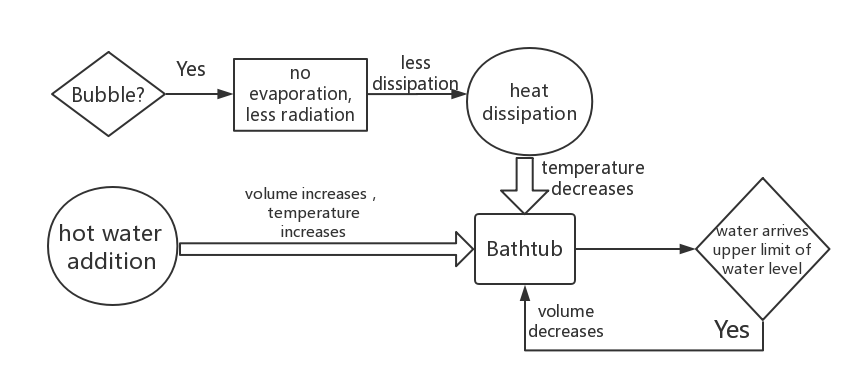
\includegraphics[height=7cm]{process.png}}
\caption{the process of simulation}                  %流程图
\label{oval}	
\end{figure}

\subsection{model testing}			%6.2 model test
\indent First, we need to verify the accuracy of the heat dissipation model.
We want to verify whether the model of the temperature change over time is in accordance with the actual situation.\\
\indent We set the bath time as half an hour. And we don't add hot water or bubble bath additive in the bathtub. \\
\begin{figure}[H]
\centerline{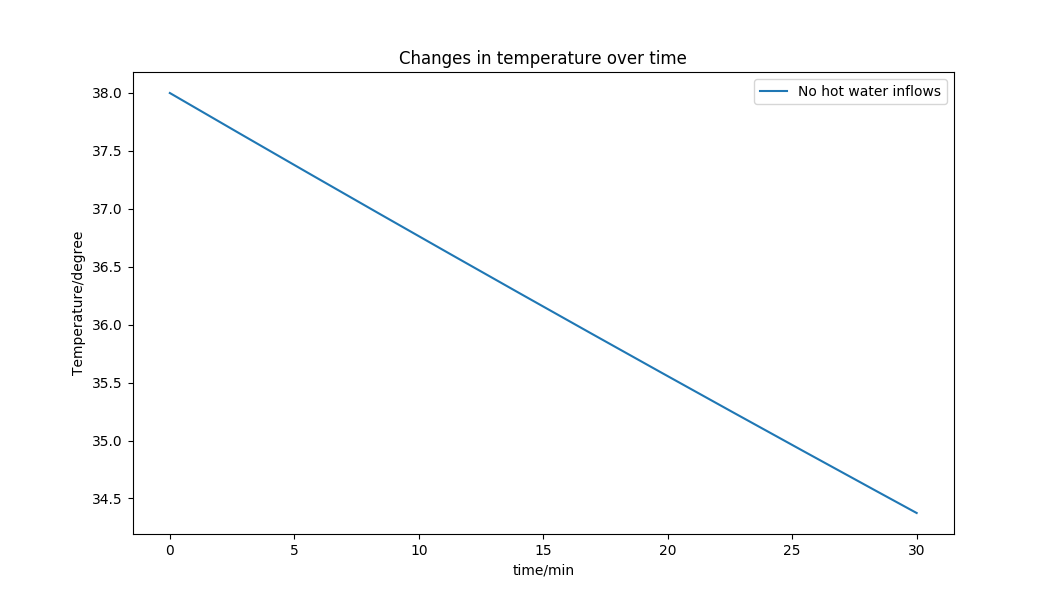
\includegraphics[height=9cm]{Figure_1-0.png}}
\caption{changes in temperature over time}
\label{oval}	
\end{figure}
\indent The model implementation with computer is shown in the figure.
We can get that the temperature in the bathtub has fallen as time goes on.It drops 4.5$^{\circ}C$ as half an hour in the bathtub. And in the indoor environment, we find the temperature of most bathtub without constant temperature system drops from 3 to 5$^{\circ}C$ in half an hour. \\ \indent Our results is within this range. So the model fits the reality.               
	%模型的检验,没有加热水时候浴缸内水温度降低的趋势符合现实
\subsection{solve the model}%模型的求解,找到一个适合的值,使水温变化小
\indent As we mentioned in the model of hot water addition, when the inflow of water per unit time changes, the heat that the bathtub get is different. So we can change the amount of inflowing water during unit time to make the temperature of bathtub different.\\ 
\indent We want to find a water inflowing per unit time which make the temperature is kept near the initial temperature of the bathtub. 
So we use the minimum dichotomy by constantly changing the amount of inflowing water during unit time. \\			
		%假装自己使用了二分法来找这个值
\indent And finally we found the water inflowing per unit time through more than a dozen iterations as $V_{best}$.\\
\begin{equation}
	V_{best}=40ml/s
\end{equation}
\indent The figure below shows the image of temperature varying with time when hot water is added.
\begin{figure}[H]	%图1.3
\centerline{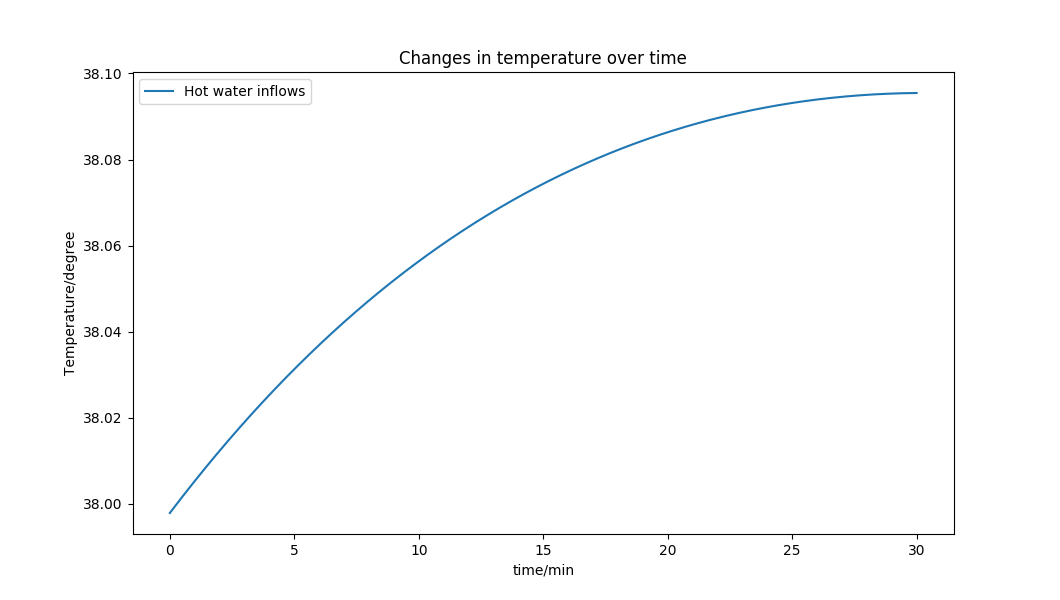
\includegraphics[height=8cm]{Figure_1-3.png}}
\caption{temperature varying with time when hot water is added}
\label{oval}	
\end{figure}
\indent When hot water is added at in $V_{best}$, the temperature will only change in a very small range from 38 to 38.09. So we get a result that the fluctuation of the temperature is always kept in a range from 0 to 0.1. \\
\indent It means the temperature will nearly not change.\\
%温度下降和温度稳定的比较
\indent Next, we want to find what is the result of adding hot water as $V_{best}$ to the model. So we made a comparison between temperature varying with time when hot water is added and not added. As shown in the picture:
\begin{figure}[H]	%图1.1
\centerline{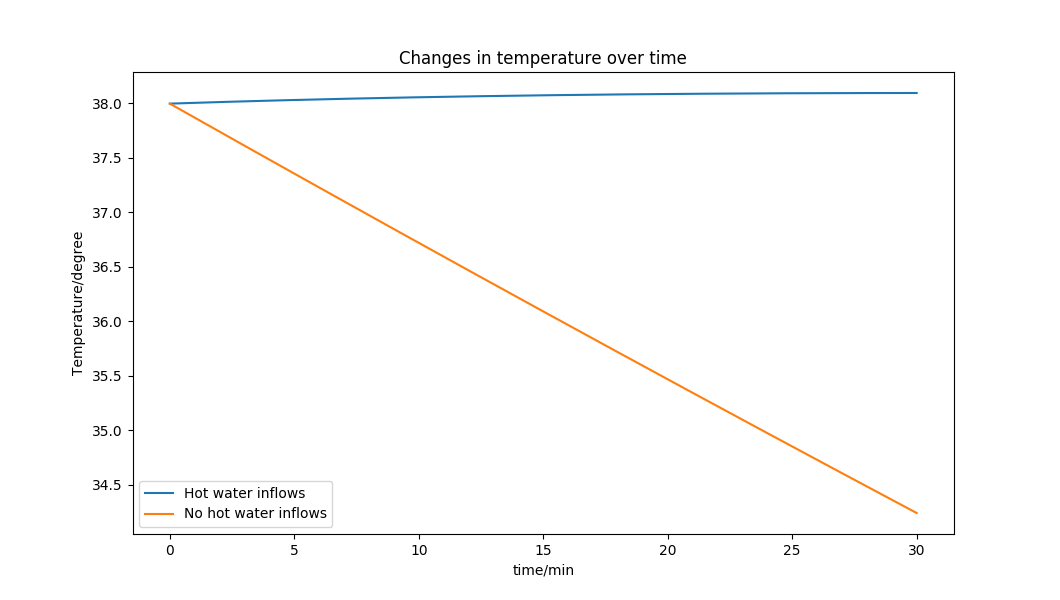
\includegraphics[height=8cm]{Figure_1-4.png}}
\caption{changes in temperature over time}
\label{oval}	
\end{figure}
\indent The curves tell that our hot water is set perfectly, the temperature will neither get too high nor get too low. \\
\indent When the water inflowing per unit time is $V_{best}$. We got a result that the fluctuation of the temperature is always kept in a range from $0$ to $0.1$. And the goal of keeping the temperature as close as possible to the initial temperature is achieved.
\subsection{model optimization}
\indent It can be obtained from the above that when we use the minimum dichotomy to find the $V_{best}$,  there always have a range from $0$ to $0.1$. It may bring some error. And we want to minimize the error of the model as we can. So we try to use the simulated annealing algorithm to optimize our model. 
\subsubsection{simulated annealing algorithm}
\indent Starting from a higher initial temperature, the simulated annealing algorithm randomly searches for the global optimal solution of the objective function in the solution space with the sudden drop of the temperature parameter. In other words, the local optimal solution can jump out of probability Eventually tends to the global optimum.
\subsubsection{Optimization results}
\indent We use python to implement simulated annealing algorithm.We call library functions of simulated annealing algorithm optimize our model. Finally, we successfully optimize our model and made the range of the $V_{best}$ get less. As shown in the picture:
\begin{figure}[H]	%图1.3
\centerline{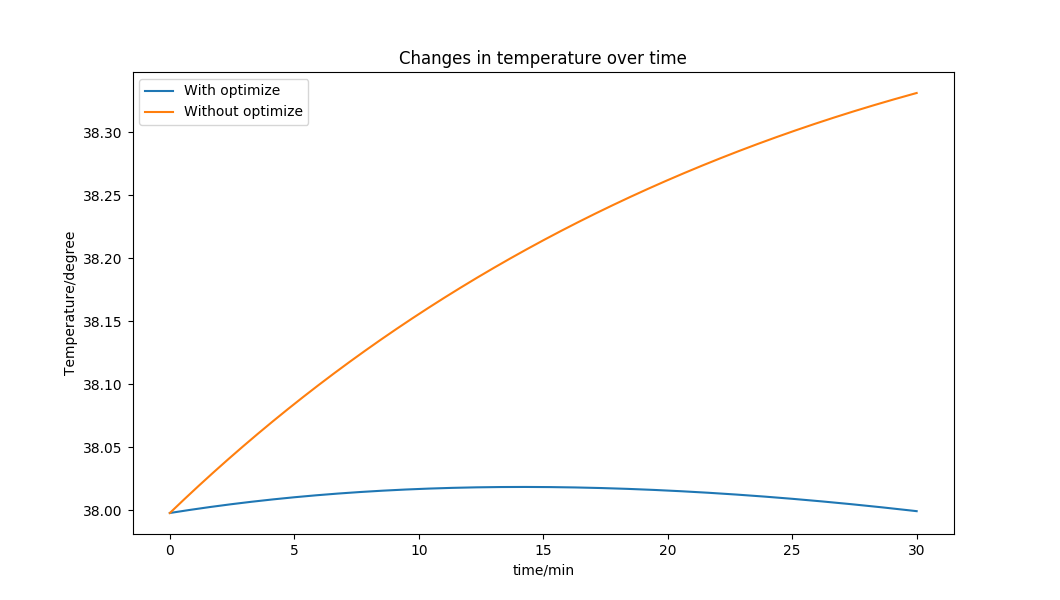
\includegraphics[height=8cm]{Figure_3-1.png}}
\caption{temperature varying with time when optimized}
\label{oval}	
\end{figure}
\indent We can find that the curve of temperature with optimization approximately coincides with another curve without optimization. We got two curves with less variance. So The fluctuation of the temperature gets smaller. We successfully optimize our model.
\subsection{Verifying the stability of the model}%验证模型的稳定性
\indent In real life, everyone's bath time is different. We should consider that some persons want to bath for longer time. So we should prolong the abscissa with more bath time to verify the stability of the model.\\
\indent We prolong the bath time to 150 minutes. The figure below shows the change when time prolong.
\begin{figure}[H]	%图1.3
\centerline{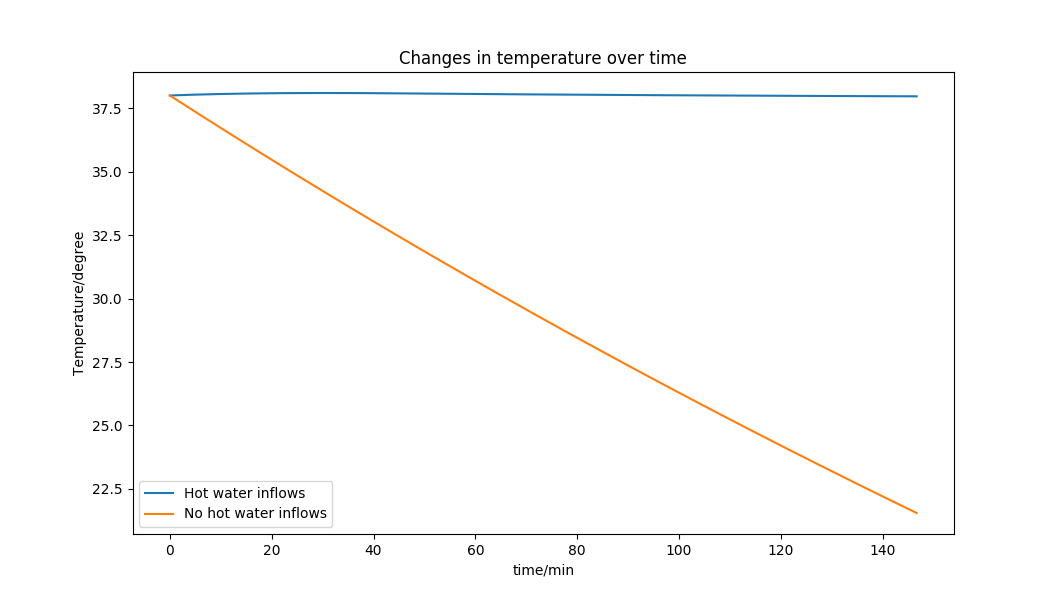
\includegraphics[height=8cm]{Figure_1-1.png}}
\caption{temperature varying with time when hot water is added}
\label{oval}	
\end{figure}
\indent Therefore, when hot water is not added, the temperature will decrease with time constantly, even the temperature will be lower than the room temperature set previously.
But when hot water is added, the temperature can also be kept well. So our model is stable and effective.

%Section 7
\section{Factors that affect the model}
\subsection{Different shapes of the bathtub}
We model and analysis several different shapes of bathtubs.
\subsubsection{Bathtub based on ovals}
\begin{figure}[H]
\centerline{\includegraphics[height=8cm]{oval.png}}
\caption{The shape of bathtub based on ovals}
\label{oval}	
\end{figure}
The elliptical long axis on the bottom of the bathtub is $A$, the short axis is $B$, the height of the whole bathtub is $h$, and the lower bottom long axis is $A-2d$.\\
\indent We divide the bathtub into an infinite number of elliptical columns with a height of $dz$, with a long semi-axis of each elliptical element\\
\begin{equation}
a(z)=\frac{A}{2}-d+\frac{d}{{H}^{2}}{z}^{2}
\end{equation}
\indent Short semi-axis of each elliptical element is
\begin{equation}
b(z)=\frac{B}{2}-d\frac{B}{A}+\frac{Bd}{A{H}^{2}}{z}^{2}
\end{equation}\\
\textbf{Calculation of the volume of water} \\\\
\indent The volume of the small cylinder is
\begin{equation}
dV=Sdz=\pi a(z)b(z)
\end{equation}
\indent The relationship between the volume of water in the bathtub and the height of the liquid surface is
\begin{equation}
\begin{split}
V(h)&=\int dV=\int Sdz=\int_{0}^{h}\pi a(z)b(z)dz \\
&=\int_{0}^{h}\pi(\frac{A}{2}-d+\frac{d{z}^{2}}{{H}^{2}})(\frac{B}{2}-d\frac{B}{A}+\frac{dB{z}^{2}}{A{H}^{2}})dz
\label{V}
\end{split}
\end{equation}
\indent We can get relationship between the volume of water and the height of liquid surface by replacing the bathtub size into the formula (\ref{V}).\\\\
\textbf{Calculation of the contact area of water with the bathtub and air} \\\\
\indent Without considering the effect of person, the upper and lower surface of the liquid contact are standard ovals.\\
\indent The area of upper surface is\\
\begin{equation}
S_{1}=\frac{\pi AB}{4}
\end{equation}
\indent And area of the lower surface is\\
\begin{equation}
	S_{2}=\pi (\frac{A}{2}+(\frac{h^{2}}{H^{2}}-1)d)(\frac{B}{2}+(\frac{h^{2}}{H^{2}}-1)d\frac{B}{A})
\end{equation}
\indent In order to calculate the contact area between the liquid and side of the bathtub, we use the calculus method.\\
\indent The area of the small cylinder is 
\begin{equation}
ds=\sqrt{1+(\frac{\partial a(z)}{\partial z}^{2})} L(z)
\label{ds}
\end{equation}
\indent where $a(z)$ is the long axis of a cross section ellipse with a height of $h$ and $L(x)$ is the circumference of the ellipse of the cross section. And $L(x)$ is
\begin{equation}
L(z)=\pi (\frac{3}{2}(a(z)+b(z))-\sqrt{a(z)b(z)})
\end{equation} 
\indent So we can get the lateral area through the integral (\ref{ds})
\begin{equation}
	S_{3}=\int ds=\int_{0}^{h}\pi \sqrt{1+\frac{4d^{2}z^{2}}{h^{4}}}(\frac{3}{2}(a(z)+b(z))-\sqrt{a(z)b(z)})dz
\end{equation}

\subsubsection{Bathtub based on circles}
\begin{figure}[H]
\centerline{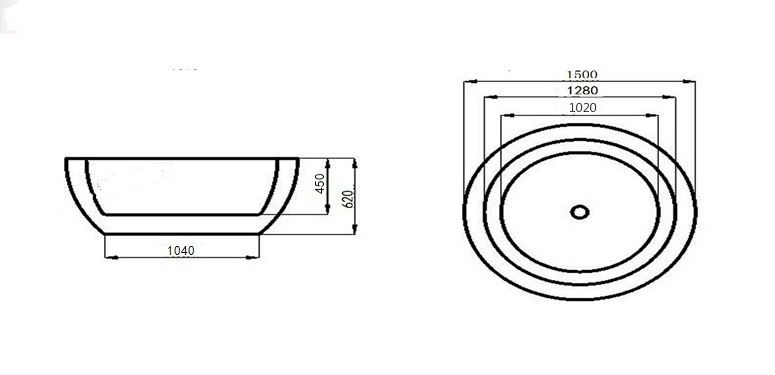
\includegraphics[height=8cm]{circle.png}}
\caption{The shape of bathtub based on circles}
\label{circle}	
\end{figure}
\indent Also without considering the effect of person, the upper and lower surface of the liquid contact are standard ovals.\\
\indent The area of upper surface is\\
\begin{equation}
S_{1}=\pi (R+(\frac{h^{2}}{H^{2}}-1)d)^{2}
\end{equation}
\indent And area of the lower surface is\\
\begin{equation}
S_{2}=\pi (R-d)^{2}
\end{equation}
\indent where $R$ is the upper surface area of the bathtub, $H$ is the height of bathtub, $d$ is the the difference between the radius of the upper surface and the lower surface, and $h$ is the height of the liquid surface.\\ 
\indent In order to calculate the contact area between the liquid and side of the bathtub, we use the calculus method like the oval-based bathtub.\\
And we can get the area of side surface $S_{3}$ of the bathtub.
\begin{equation}
	S_{3}=\int ds=\int_{0}^{h}\pi \sqrt{1+\frac{4d^{2}z^{2}}{h^{4}}}({3}r(z))-r(z))dz
\end{equation}
\indent where $r(z)$ is
\begin{equation}
	R+(\frac{h^{2}}{H^{2}}-1)d
\end{equation}
\\\\
\noindent\
\textbf{Simulation Result}\\\\
\indent We compare two ways of adding hot water. And when  
\begin{figure}[H]
	\centerline{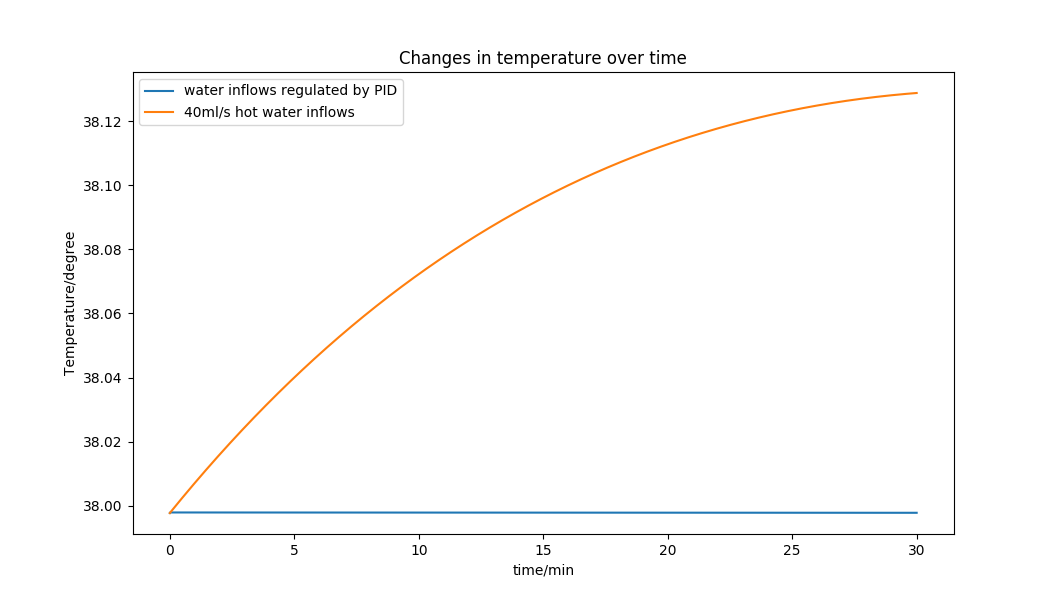
\includegraphics[height=10cm]{Figure_4-2.png}}
	\caption{Comparison of two kinds of water adding methods}
	\label{circle}	
\end{figure}

\subsection{The effect of human body and body temperature on the model}
%subsection 4.1
We improved our model in view of the human body influence. Our improvement is mainly in the following aspects.
\subsubsection{The influence of the heat conduction}%sub subsection 4.1.1
The interior of the body is basically maintained at a constant temperature, and the temperature of the skin is close to the water in bathtub. So we can simplify the question.The simplified question is illustrated as floows.\\

\begin{figure}[H]
\centerline{\includegraphics[height=6cm]{skin.png}}
\caption{Heat conduction model of human body}
\label{skin}
\end{figure}
\indent We can assume that the temperature of the skin is the same as the water. We select the temperature of the rectum about 37.5 degrees as the body temperature. The problem can be simplified as the skin heat dissipating to the interior of the body.\\
\indent So we can use {\bf Newton's law of cooling} to calculate the speed of heat dissipation.\\
\begin{equation}
\begin{split}
\Delta T&=|T_{w}-T_{f}| \\
q&=h\Delta T	\\
\phi &=qA=Ah\Delta T
\end{split}
\end{equation}
\indent Where \textbf{\emph{q}} is the heat flux density. \textbf{\emph{h}} is the convection heat transfer coefficient of matter. \textbf{\emph{$\phi$}}  is heat transfer power (or heat transfer per unit time). \textbf{\emph{A}} is the heat transfer area.\\
\indent The surface area of the human body can be calculated by the following formula.
\begin{equation}
S= \begin{cases} & 0.0057*h+0.0121*w+0.0820\text{( man )} \\ & 0.0073*h+0.0127*w-0.2106\text{(woman)} \end{cases}
\label{s}
\end{equation}
\indent According to formula \ref{skin}, the quantity of heat dissipated($dQ$) in unit time is:
\begin{equation}
	\frac{\mathrm{d} Q}{\mathrm{d} t}=\phi =qA=Sh\Delta T
	\label{Q_skin}
\end{equation}
where \emph{h}=1.48,${T_{f}}=37.5^{\circ}$. \\
\indent We add this part of heat loss to our heat dissipation model. The change of temperature with time is obtained by the simulation program. And the result is drawn into a graph as follows
\begin{figure}[H]
	\centerline{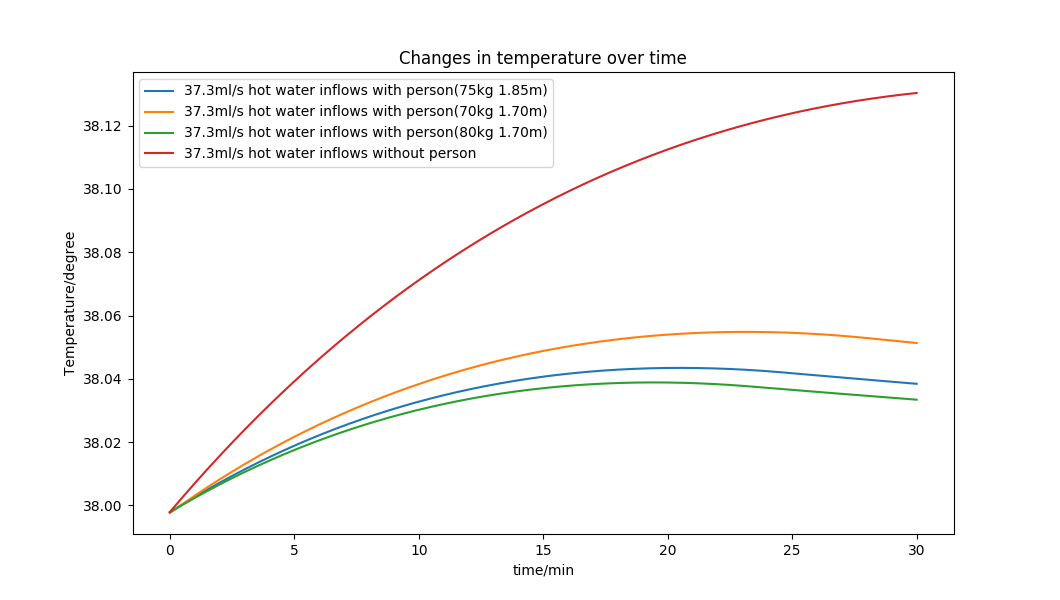
\includegraphics[height=10cm]{Figure_4-5.png}}
	\caption{The change of temperature influenced by human body over time}
	\label{s_person}	
\end{figure}
\subsubsection{The influence of the body shape and action}
The volume of the person in the water affects the height of the liquid. In order to discuss the influence on the liquid surface conveniently. We use the weight to estimate the volume of the body. We use $\rho =1.06\times10^{3}kg/m^{3}$ as the density of the human body, so the volume can be calculated:
\begin{equation}
v_{body}=\frac{m}{\rho }=\frac{m}{1.06\times 10^{3}}(m^{3})
\end{equation}
\indent If we consider the effect of the body volume, we need to correct of the height of the liquid surface. We assume 65\% volume of the body is in the water. So the height of the liquid surface should be corrected to\\
\begin{equation}
	h=H(v_{water}+0.65v_{body})
\end{equation}
\indent Because the effect of body action on convection and radiation heat dissipation is very small, we simplify the effect of body action on our model.\\
\indent We assume that the movements of persons can only lead to a water spill that is equivalent to a certain proportion of the body's volume. We set the volume of liquid for each overflow is $dv$
\begin{equation}
	dv=5\times10^{-3}v_{body}
\end{equation}
\indent We set the probability of water overflow per second is 0.02, which means there is an overflow of water on average in half a minute.\\\\
\noindent
\textbf{Simulation Result}\\\\
\indent We model the model with the added action impact model and compare it with the simulation results that have no action impact, and we get the following figure
\begin{figure}[H]
	\centerline{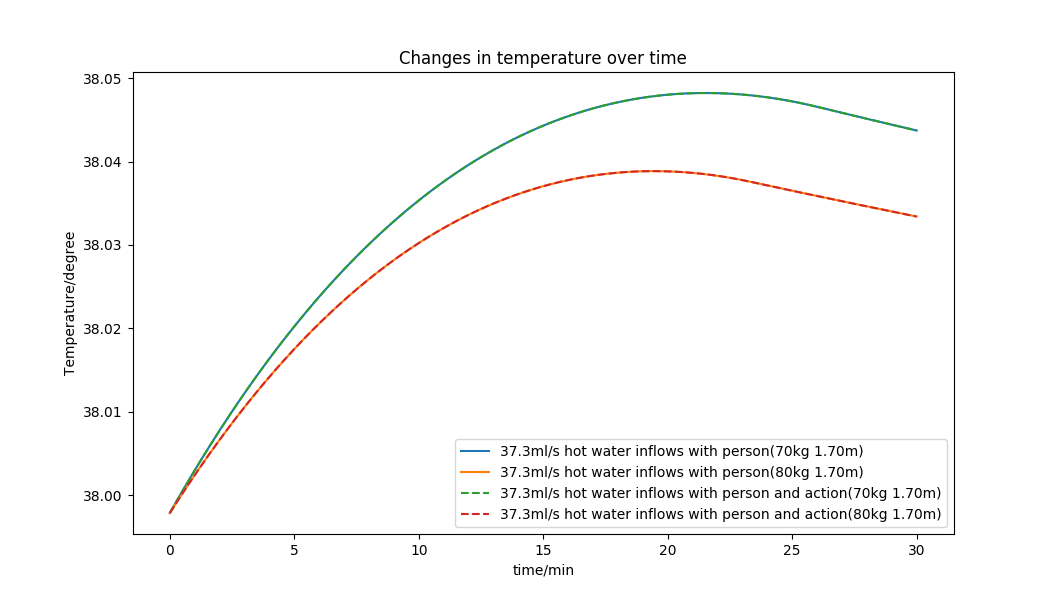
\includegraphics[height=10cm]{Figure_4-6.png}}
	\caption{The effect of body action}
	\label{action}	
\end{figure}
\indent By analyzing the Figure \ref{action}, we can find that the action and no action curve basically coincide. Therefore, the action has little effect on the trend of temperature change.
\begin{table}[H]
	\setlength{\abovecaptionskip}{0pt}
	\setlength{\belowcaptionskip}{0pt}
	\centering{Table 3:The simulation result}\\
	\begin{tabular}{p{2cm}|p{2cm}|p{1.5cm}|p{3cm}|p{1cm}|p{2cm}}
		\hline
		\rowcolor[gray]{0.9}\bf{water flow}	&\bf{Water consumption} &\bf{bubble}&\bf{body shape}&\bf{action}&\bf{temperature variance} \\
		\hline
		PID 	 & 68.838L &No  &No &No &0.007026\\
		40.0ml/s   & 72.000L &No  &No &No &15.66907\\
		\hline
		PID 	 & 64.006L &Yes &No &No &0.007026\\
		40.0ml/s   & 72.000L &Yes &No &No &86.95530\\
		\hline
		37.3ml/s & 67.140L &Yes &No &No &15.61321\\
		37.3ml/s & 67.140L &Yes &75kg 1.85m &Yes &2.242\\	
		37.3ml/s & 67.140L &Yes &70kg 1.70m &Yes &3.612\\
		37.3ml/s & 67.140L &Yes &80kg 1.70m &Yes &3.279\\
		\hline
		PID & 64.006L &Yes &No &No &0.00702\\
		PID & 66.167L &Yes &75kg 1.85m &Yes &0.00750\\	
		PID & 66.042L &Yes &70kg 1.70m &Yes &0.00747\\
		PID & 66.286L &Yes &80kg 1.70m &Yes &0.00753\\
		\hline
	\end{tabular}
\end{table}
\section{Sensitivity analysis}
\subsection{Selection of indictors}%subsection 6.1
\subsection{Selection of aggregation method}%subsection 6.2
\section{Strengths and Weaknesses}
\subsection{Strengths}
\begin{itemize}
\item{\textbf{The simulation result of our model is appealing.} As we have shown before, almost all the simulation of our model is according with the real world situation. And this means our model is effective to describe the process of bath.}
\item{\textbf{Our model is steady.} When the different influential factors are considered, our model is still effective. Our model is steady to describe the process in a varied situation. }
\item{\textbf{Our model is easy to implement.} We give the specific amount of inflowing water. When the real environmental parameters are given, the users can easily adjust the amount of inflowing water to keep the initial temperature. }
\end{itemize}
\subsection{Weaknesses}
\begin{itemize}
\item{\textbf{The motions of people is simplified.}The motions of people are too complicated and variable to consider. Some complicated motions may bring more influence on our model. }
\end{itemize}


\section{References}
\begin{thebibliography}{99}
\bibitem{1}Bannerjee,S.Bone,J.and Finger,Y.(2016).European Digital City Index-Methodology Report.Nesta Report-ISBN Number:978-1-84875-153-8
\end{thebibliography}

\begin{appendices}
\end{appendices}

\end{document}